%!TEX root = ../presentation.tex 


\section{Bonnes pratiques des composantes \& BOM}

\subsection{Footprints}
\begin{frame}{Fabrication du footprint}
    \begin{twocolumns}
        \leftcol
        \begin{itemize}
            \item Élément très important de la conception de pièces
            \item Affecte le layout et l'assemblage
            \bigskip
            \item Le footprint devrait être clair
            \item Le footprint devrait être représentatif
            \item Le footprint devrait avoir des bonnes informations mécaniques
            \item Le footprint devrait respecter tes capacités d'assemblage
            \item Le footprint devrait avoir un modèle 3D
        \end{itemize}

        \rightcol
        \begin{itemize}
            \item Faire le footprint soi-même
            \begin{itemize}
                \item Suivre un standard
                \item Modifier la pièce plus tard au besoin
                \item Avoir des marqueurs de pin 1 consistants
                \item Avoir les bonnes couches mécaniques
                \item Avoir des bons modèles 3D
                \item Valider que le footprint est bon
            \end{itemize}
        \end{itemize}
    \end{twocolumns}
\end{frame}

\begin{frame}{Attention aux footprints!}
    \begin{twocolumns}
        \leftcol
        \begin{itemize}
            \item Toujours valider tous les footprints
            \item Faire attention aux sources de footprints
            \item Faire attention particulière aux transistors!
            \bigskip
            \item La meilleure option est de faire le footprint
        \end{itemize}
        \rightcol
        \makefigure[1][0.25][Microchip LND150]{transistor-lnd150-sgd}
        \makefigure[1][0.25][Vishay SQ2318]{transistor-sq2318-dgs}
    \end{twocolumns}
\end{frame}

\begin{frame}{Marqueurs de pin 1}
    \begin{twocolumns}
        \leftcol
        \only<1-2>{
            \begin{itemize}
                \item Doit être visible clairement pendant l'assemblage
                \begin{itemize}
                    \item Couche d'assemblage avec les marqueurs
                \end{itemize}
                \item Doit être visible après l'assemblage!
                \item Plusieurs marqueurs possibles
            \end{itemize}
        }
        \only<3->{
            \makefigureborder[0.75][0.7]{footprint-qfn32-5x5}
        }
        \rightcol
        \only<1-2>{
            \tcbox[colframe=accent, colback=background]{
                \begin{tikzpicture}
                    \node[anchor=south west, inner sep=0] at (0,0) {
                        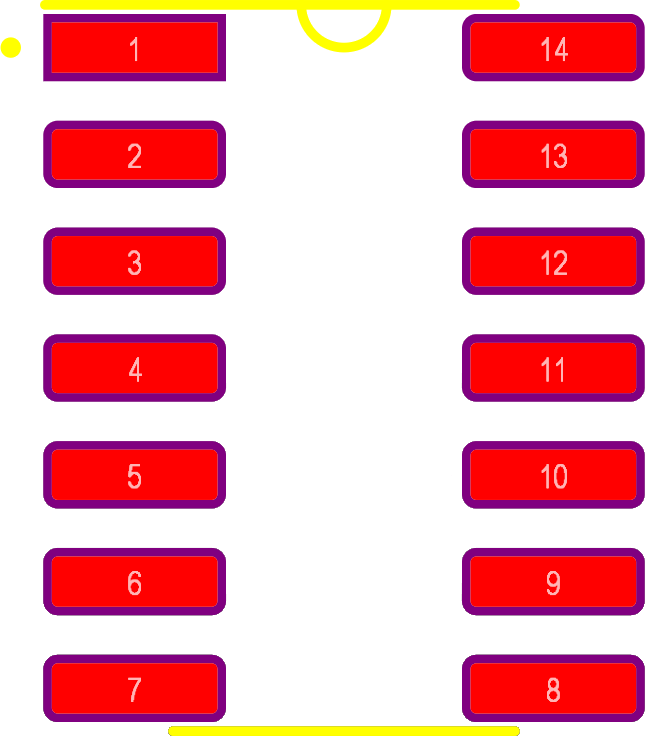
\includegraphics[width=0.75\textwidth,
                                         height=0.7\textheight,
                                         keepaspectratio]{
                            pictures/footprint-soic14-3_8mm}};
                    \only<2>{
                        \draw[accent, ultra thick, rounded corners] (-0.15, 5.35) rectangle (0.3, 5.8);
                        \draw[accent, ultra thick, rounded corners] (0.3, 5.8) rectangle (2, 6.1);
                        \draw[accent, ultra thick, rounded corners] (2.25, 5.35) rectangle (3.35, 6.1);
                        \draw[accent, ultra thick, rounded corners] (1.5, 5.25) rectangle (2, 5.5);
                    }
                \end{tikzpicture}
            }
        }
        \only<3->{
            \makefigureborder[0.75][0.7]{footprint-tssop20-4_4mm}
            }
    \end{twocolumns}
\end{frame}

% TODO: Couches mécaniques
% S'assurer de respecter les couches mécaniques

\subsection{Symboles}

\begin{frame}{Fabrication du symbole}
    \begin{twocolumns}[0.6]
        \leftcol
        \begin{itemize}
            \item Un des éléments de clareté les plus importants
            \item Affecte aussi le BOM
            \bigskip
            \item La pièce devrait être représentative
            \item La pièce devrait être facile à lire
            \item La pièce devrait contenir toutes les informations pour le BOM
            \bigskip
            \item Faire la pièce soi-même
            \begin{itemize}
                \item Suivre un standard
                \item Modifier plus tard pour fitter le schéma
                \item Customize le BOM
                \item Validation de la pièce
                \item Mettre les types électriques
            \end{itemize}
        \end{itemize}

        \rightcol
        \makefigure[1][0.8][Source: \cite{kicad-symbol}]{kicad-pin-electrical-type}
    \end{twocolumns}
\end{frame}

\begin{frame}{Pinout du symbole}
    \begin{itemize}
        \item Garder les inputs à gauche et outputs à droite
        \item Ne pas numéroter le symbole comme le footprint
        \item Utiliser des symboles représentatifs lorsque possible
        \item Tu ne devrais pas avoir à aller dans la datasheet pour comprendre la pièce
    \end{itemize}
    \vfill
    \only<2-> {
    \begin{columns}
        \only<2> {
        \begin{column}{\textwidth}
        }
        \only<3> {
        \begin{column}{0.5\textwidth}
        }
        \only<4-> {
        \begin{column}{0.3\textwidth}
        }
            \begin{maketikzfigure}[1][0.4]
                \only<1-4>{
                \draw (0, 0) node
                   [dipchip,
                    num pins = 8,
                    %hide numbers,
                    external pins width=0.3,
                    external pad fraction=4,
                    anchor=bpin 1,
                    thick](op){\scriptsize OPA1632};
                }
                \only<5->{
                \draw (0, 0) node
                   [dipchip,
                    num pins = 8,
                    %hide numbers,
                    external pins width=0.3,
                    external pad fraction=4,
                    anchor=bpin 1,
                    thick, color=red](op){\scriptsize OPA1632};
                }
                \node [left,  font=\tiny] at (op.pin 1) {$V_{IN_-}$};
                \node [left,  font=\tiny] at (op.pin 2) {$V_{OCM}$};
                \node [left,  font=\tiny] at (op.pin 3) {$V_+$};
                \node [left,  font=\tiny] at (op.pin 4) {$V_{OUT_+}$};
                \node [right, font=\tiny] at (op.pin 5) {$V_{OUT_-}$};
                \node [right, font=\tiny] at (op.pin 6) {$V_-$};
                \node [right, font=\tiny] at (op.pin 7) {$EN$};
                \node [right, font=\tiny] at (op.pin 8) {$V_{IN_+}$};
            \end{maketikzfigure}
            \only<5-> {
                \begin{center}
                    \textcolor{red}{\textbf{BAD}}
                \end{center}
            }
        \end{column}

        \only<3> {
        \begin{column}{0.5\textwidth}
        }
        \only<4-> {
        \begin{column}{0.3\textwidth}
        }
        \only<3-> {
            \begin{maketikzfigure}[1][0.4]
                \only<1-4>{
                \draw (0, 0) node
                   [dipchip,
                    num pins = 8,
                    hide numbers,
                    external pins width=0.3,
                    external pad fraction=4,
                    anchor=bpin 1,
                    thick](op){\scriptsize OPA1632};
                }
                \only<5->{
                \draw (0, 0) node
                   [dipchip,
                    num pins = 8,
                    hide numbers,
                    external pins width=0.3,
                    external pad fraction=4,
                    anchor=bpin 1,
                    thick, color=blue](op){\scriptsize OPA1632};
                }
                \node [left,  font=\tiny] at (op.pin 1) {$V_{OCM}$};
                \node [right, font=\tiny] at (op.bpin 1) {$2$};
                \node [left,  font=\tiny] at (op.pin 2) {$V_{IN_+}$};
                \node [right, font=\tiny] at (op.bpin 2) {$8$};
                \node [left,  font=\tiny] at (op.pin 3) {$V_{IN_-}$};
                \node [right, font=\tiny] at (op.bpin 3) {$1$};
                \node [left,  font=\tiny] at (op.pin 4) {$EN$};
                \node [right, font=\tiny] at (op.bpin 4) {$7$};
                \node [right, font=\tiny] at (op.pin 5) {$V_-$};
                \node [left,  font=\tiny] at (op.bpin 5) {$6$};
                \node [right, font=\tiny] at (op.pin 6) {$V_{OUT_-}$};
                \node [left,  font=\tiny] at (op.bpin 6) {$5$};
                \node [right, font=\tiny] at (op.pin 7) {$V_{OUT_+}$};
                \node [left,  font=\tiny] at (op.bpin 7) {$4$};
                \node [right, font=\tiny] at (op.pin 8) {$V_+$};
                \node [left,  font=\tiny] at (op.bpin 8) {$3$};
            \end{maketikzfigure}
            \only<5-> {
                \begin{center}
                    \textcolor{blue}{\textbf{GOOD}}
                \end{center}
            }
        \end{column}
        }

        \only<4-> {
        \begin{column}{0.4\textwidth}
            \begin{maketikzfigure}[1][0.4]
                \only<1-4>{
                \draw (0, 0) node[fd op amp,
                                  thick, font=\normalsize,
                                  xscale=2, yscale=2,
                                  component text=left](op){\tiny OPA1632};
                }
                \only<5->{
                \draw (0, 0) node[fd op amp,
                                  thick, font=\normalsize,
                                  xscale=2, yscale=2,
                                  component text=left, color=accent](op){\tiny OPA1632};
                }
                \node[left,  font=\normalsize, label =15:{\scriptsize 8}] at (op.+)       {$V_{IN_+}$};
                \node[left,  font=\normalsize, label =15:{\scriptsize 1}] at (op.-)       {$V_{IN_-}$};
                \node[right, font=\normalsize, label=195:{\scriptsize 5}] at (op.out -)   {$V_{OUT_-}$};
                \node[right, font=\normalsize, label=165:{\scriptsize 4}] at (op.out +)   {$V_{OUT_+}$};
                \node[left,  font=\normalsize, label =15:{\scriptsize 2}] at (-2.4, 0)    {$V_{OCM}$};
                \node[left,  font=\normalsize, label =15:{\scriptsize 2}] at (-2.4, -2.4) {$EN$};

                \only<1-4>{
                    \draw[thick]
                    (-2.4, 0) to [short] (op.leftedge)
                    (op.up)   to (op.up   |- 0, 2)  node[vcc, font=\normalsize, label=285:{\scriptsize 3}] {$V_+$}
                    (op.down) to (op.down |- 0, -2) node[vee, font=\normalsize, label=105:{\scriptsize 6}] {$V_-$}
                    (-2.4, -2.4) to [short] (-1, -2.4) to [short] (-1, -1.6)
                    ;
                }
                \only<5->{
                    \draw[thick, color=accent]
                    (-2.4, 0) to [short] (op.leftedge)
                    (op.up)   to (op.up   |- 0, 2)  node[vcc, font=\normalsize, label=285:{\scriptsize 3}] {$V_+$}
                    (op.down) to (op.down |- 0, -2) node[vee, font=\normalsize, label=105:{\scriptsize 6}] {$V_-$}
                    (-2.4, -2.4) to [short] (-1, -2.4) to [short] (-1, -1.6)
                    ;
                }
            \end{maketikzfigure}
            \only<5-> {
                \begin{center}
                    \textcolor{accent}{\textbf{BEST}}
                \end{center}
            }
        \end{column}
        }
    \end{columns}
    }
\end{frame}

\begin{frame}{Symboles représentatifs}
    \begin{columns}
        \only<1>{
        \begin{column}{\textwidth}
        }
        \only<2->{
        \begin{column}{0.5\textwidth}
        }

        \only<1-2>{
            \begin{maketikzfigure}[1][0.8]
                \draw
                (0, 0) to [short, l={$ENABLE$}] (2, 0) to [R] (4, 0)
                to [full led, color=accent] (6, 0);
                \draw
                (0, -2) to [short, l={$POWER GOOD$}] (2, -2) to [R] (4, -2)
                to [full led, color=accent] (6, -2);
                \draw
                (0, -4) to [short, l={$STATUS$}] (2, -4) to [R] (4, -4)
                to [full led, color=red] (6, -4);
                \draw
                (0, -6) to [short, l={$HEARTBEAT$}] (2, -6) to [R] (4, -6)
                to [full led, color=orange] (6, -6);
                \draw
                (6, 0) to [short] (6, -7) node[ground, xscale=2, yscale=2]{};
            \end{maketikzfigure}
        }


        \only<3-4>{
            \ctikzset{multipoles/dipchip/width=2}
            \ctikzset{diodes/scale=0.5}
            \begin{maketikzfigure}[1][0.8]
                \draw (0, 0) node
                   [dipchip,
                    num pins = 12,
                    hide numbers, no topmark,
                    external pins width=0.3,
                    external pad fraction=4,
                    draw only pins={1, 3-4, 6}](esd){};
                \node at ($(esd.bpin 1) + (0.825, 0.4)$) {\tiny EPD2E001DRLR};

                \node [right, font=\tiny] at (esd.bpin 1) {$VCC$};
                \node [left,  font=\tiny] at (esd.pin  1) {$1$};
                \node [right, font=\tiny] at (esd.bpin 3) {$IO1$};
                \node [left,  font=\tiny] at (esd.pin  3) {$3$};
                \node [right, font=\tiny] at (esd.bpin 4) {$IO2$};
                \node [left,  font=\tiny] at (esd.pin  4) {$5$};
                \node [right, font=\tiny] at (esd.bpin 6) {$GND$};
                \node [left,  font=\tiny] at (esd.pin  6) {$4$};


                \draw ($(esd.bpin 1) + (0.65, 0)$) to ($(esd.bpin 1) + (2.25, 0)$);
                \draw ($(esd.bpin 3) + (0.5,  0)$) to ($(esd.bpin 3) + (1, 0)$);
                \draw ($(esd.bpin 4) + (0.5,  0)$) to ($(esd.bpin 4) + (1.75, 0)$);
                \draw ($(esd.bpin 6) + (0.65, 0)$) to ($(esd.bpin 6) + (2.25, 0)$);

                \draw ($(esd.bpin 3) + (1, 0)$) to
                      [full diode] ($(esd.bpin 1) + (1, 0)$);
                \draw ($(esd.bpin 4) + (1.75, 0)$) to
                      [short] ($(esd.bpin 3) + (1.75, 0)$) to
                      [full diode] ($(esd.bpin 1) + (1.75, 0)$);

                \draw ($(esd.bpin 6) + (1, 0)$) to 
                      [full diode] ($(esd.bpin 4) + (1, 0)$) to
                      [short] ($(esd.bpin 3) + (1, 0)$);
                \draw ($(esd.bpin 6) + (1.75, 0)$) to 
                      [full diode] ($(esd.bpin 4) + (1.75, 0)$);

                \draw ($(esd.bpin 6) + (2.25, 0)$) to
                      [full ZZener diode] ($(esd.bpin 1) + (2.25, 0)$);
            \end{maketikzfigure}
        }
        \only<5->{
            \ctikzset{multipoles/dipchip/width=2}
            \begin{maketikzfigure}[1][0.8]
                \draw (0, 0) node
                   [dipchip,
                    num pins = 12,
                    hide numbers, no topmark,
                    external pins width=0.3,
                    external pad fraction=4,
                    draw only pins={1, 3, 5-6, 7-8, 10, 12}](reg){};
            \node at ($(reg.bpin 1) + (0.825, 0.4)$) {\tiny LMZ23605TZE};

            \node [right, font=\tiny] at (reg.bpin 1) {$V_{IN}$};
            \node [left,  font=\tiny] at (reg.pin  1) {$1$};
            \node [right, font=\tiny] at (reg.bpin 3) {$EN$};
            \node [left,  font=\tiny] at (reg.pin  3) {$3$};
            \node [right, font=\tiny] at (reg.bpin 5) {$SYNC$};
            \node [left,  font=\tiny] at (reg.pin  5) {$2$};
            \node [right, font=\tiny] at (reg.bpin 6) {$SS$};
            \node [left,  font=\tiny] at (reg.pin  6) {$6$};

            \node [left,  font=\tiny] at (reg.bpin 7)  {$PGND$};
            \node [right, font=\tiny] at (reg.pin  7)  {$8$};
            \node [left,  font=\tiny] at (reg.bpin 8)  {$AGND$};
            \node [right, font=\tiny] at (reg.pin  8)  {$4$};
            \node [left,  font=\tiny] at (reg.bpin 10) {$FB$};
            \node [right, font=\tiny] at (reg.pin  10) {$5$};
            \node [left,  font=\tiny] at (reg.bpin 12) {$V_{OUT}$};
            \node [right, font=\tiny] at (reg.pin  12) {$7$};

            \end{maketikzfigure}
        }
        \end{column}

        \only<2-3>{
        \begin{column}{0.5\textwidth}
            \ctikzset{multipoles/dipchip/width=5}
            \begin{maketikzfigure}[1][0.8]
                \draw (0, 0) node
                   [dipchip,
                    num pins = 40,
                    hide numbers, no topmark,
                    external pins width=0.3,
                    external pad fraction=4,
                    draw only pins={1, 2, 4-5, 10, 11, 17, 18, 20, 21-22, 24-25, 27-28, 30-31, 33-34, 36-37, 39-40},
                    thick](adc){};
                \node at ($(adc.bpin 1) + (1.65, 0.5)$) {\textbf{ADS62P48IRGCT}};

                \node [right] at (adc.bpin 1) {$DVDD$};
                \node [left]  at (adc.pin  1) {$1$};
                \node [right] at (adc.bpin 2) {$AVDD$};
                \node [left]  at (adc.pin  2) {$16$};

                \node [right] at (adc.bpin 4) {$CLK_+$};
                \node [left]  at (adc.pin  4) {$25$};
                \node [right] at (adc.bpin 5) {$CLK_-$};
                \node [left]  at (adc.pin  5) {$26$};

                \node [right] at (adc.bpin 10) {$IN_+$};
                \node [left]  at (adc.pin  10) {$19$};
                \node [right] at (adc.bpin 11) {$IN_-$};
                \node [left]  at (adc.pin  11) {$20$};

                \node [right] at (adc.bpin 17) {$EN$};
                \node [left]  at (adc.pin  17) {$12$};
                \node [right] at (adc.bpin 18) {$RST$};
                \node [left]  at (adc.pin  18) {$15$};
                \node [right] at (adc.bpin 20) {$GND$};
                \node [left]  at (adc.pin  20) {$17$};

                \node [left]  at (adc.bpin 40) {$D0_+$};
                \node [right] at (adc.pin  40) {$61$};
                \node [left]  at (adc.bpin 39) {$D0_-$};
                \node [right] at (adc.pin  39) {$60$};
                \node [left]  at (adc.bpin 37) {$D1_+$};
                \node [right] at (adc.pin  37) {$63$};
                \node [left]  at (adc.bpin 36) {$D1_-$};
                \node [right] at (adc.pin  36) {$62$};
                \node [left]  at (adc.bpin 34) {$D2_+$};
                \node [right] at (adc.pin  34) {$3$};
                \node [left]  at (adc.bpin 33) {$D2_-$};
                \node [right] at (adc.pin  33) {$2$};
                \node [left]  at (adc.bpin 31) {$D3_+$};
                \node [right] at (adc.pin  31) {$5$};
                \node [left]  at (adc.bpin 30) {$D3_-$};
                \node [right] at (adc.pin  30) {$4$};
                \node [left]  at (adc.bpin 28) {$D4_+$};
                \node [right] at (adc.pin  28) {$7$};
                \node [left]  at (adc.bpin 27) {$D4_-$};
                \node [right] at (adc.pin  27) {$6$};
                \node [left]  at (adc.bpin 25) {$D5_+$};
                \node [right] at (adc.pin  25) {$9$};
                \node [left]  at (adc.bpin 24) {$D5_-$};
                \node [right] at (adc.pin  24) {$8$};
                \node [left]  at (adc.bpin 22) {$D6_+$};
                \node [right] at (adc.pin  22) {$11$};
                \node [left]  at (adc.bpin 21) {$D6_-$};
                \node [right] at (adc.pin  21) {$10$};

                % ADC
                \draw (-2.5, 0) to (-1.5, 1) to (-0.5, 1) to (-0.5, -1) to (-1.5, -1) to (-2.5, 0);
                \draw (adc.bpin 10 -| -2.75, 0) to (adc.bpin 10 -| -2.225, 0);
                \draw (adc.bpin 11 -| -2.75, 0) to (adc.bpin 11 -| -2.225, 0);
                \node at (-1.5, 0) {ADC};

                % DIFFERENTIAL DRIVERS
                \draw ($(adc.bpin 40) + (-1.75, 0.15)$) to ($(adc.bpin 39) + (-1.75, -0.15)$)
                to ($(adc.bpin 40) - (adc.bpin 31) + (2.5, 0)$) to ($(adc.bpin 40) + (-1.75, 0.15)$)
                ($(adc.bpin 40) - (1.485, 0)$) to ($(adc.bpin 40) - (1, 0)$)
                ($(adc.bpin 39) - (1.485, 0)$) to ($(adc.bpin 39) - (1, 0)$);

                \draw ($(adc.bpin 37) + (-1.75, 0.15)$) to ($(adc.bpin 36) + (-1.75, -0.15)$)
                to ($(adc.bpin 37) - (adc.bpin 31) + (2.5, 0)$) to ($(adc.bpin 37) + (-1.75, 0.15)$)
                ($(adc.bpin 37) - (1.485, 0)$) to ($(adc.bpin 37) - (1, 0)$)
                ($(adc.bpin 36) - (1.485, 0)$) to ($(adc.bpin 36) - (1, 0)$);

                \draw ($(adc.bpin 34) + (-1.75, 0.15)$) to ($(adc.bpin 33) + (-1.75, -0.15)$)
                to ($(adc.bpin 34) - (adc.bpin 31) + (2.5, 0)$) to ($(adc.bpin 34) + (-1.75, 0.15)$)
                ($(adc.bpin 34) - (1.485, 0)$) to ($(adc.bpin 34) - (1, 0)$)
                ($(adc.bpin 33) - (1.485, 0)$) to ($(adc.bpin 33) - (1, 0)$);

                \draw ($(adc.bpin 31) + (-1.75, 0.15)$) to ($(adc.bpin 30) + (-1.75, -0.15)$)
                to (2.5, 0) to ($(adc.bpin 31) + (-1.75, 0.15)$)
                ($(adc.bpin 31) - (1.485, 0)$) to ($(adc.bpin 31) - (1, 0)$)
                ($(adc.bpin 30) - (1.485, 0)$) to ($(adc.bpin 30) - (1, 0)$);

                \draw ($(adc.bpin 28) + (-1.75, 0.15)$) to ($(adc.bpin 27) + (-1.75, -0.15)$)
                to ($(adc.bpin 28) - (adc.bpin 31) + (2.5, 0)$) to ($(adc.bpin 28) + (-1.75, 0.15)$)
                ($(adc.bpin 28) - (1.485, 0)$) to ($(adc.bpin 28) - (1, 0)$)
                ($(adc.bpin 27) - (1.485, 0)$) to ($(adc.bpin 27) - (1, 0)$);

                \draw ($(adc.bpin 25) + (-1.75, 0.15)$) to ($(adc.bpin 24) + (-1.75, -0.15)$)
                to ($(adc.bpin 25) - (adc.bpin 31) + (2.5, 0)$) to ($(adc.bpin 25) + (-1.75, 0.15)$)
                ($(adc.bpin 25) - (1.485, 0)$) to ($(adc.bpin 25) - (1, 0)$)
                ($(adc.bpin 24) - (1.485, 0)$) to ($(adc.bpin 24) - (1, 0)$);

                \draw ($(adc.bpin 22) + (-1.75, 0.15)$) to ($(adc.bpin 21) + (-1.75, -0.15)$)
                to ($(adc.bpin 22) - (adc.bpin 31) + (2.5, 0)$) to ($(adc.bpin 22) + (-1.75, 0.15)$)
                ($(adc.bpin 22) - (1.485, 0)$) to ($(adc.bpin 22) - (1, 0)$)
                ($(adc.bpin 21) - (1.485, 0)$) to ($(adc.bpin 21) - (1, 0)$);

                % BUS
                \draw[very thick]
                (-0.5, 0) to (1.75, 0)
                (1, 0) to ($(adc.bpin 40) - (adc.bpin 31) + (1, 0)$)
                (1, 0) to ($(adc.bpin 22) - (adc.bpin 31) + (1, 0)$)
                ($(adc.bpin 40) - (adc.bpin 31) + (1, 0)$) to ($(adc.bpin 40) - (adc.bpin 31) + (1.75, 0)$)
                ($(adc.bpin 37) - (adc.bpin 31) + (1, 0)$) to ($(adc.bpin 37) - (adc.bpin 31) + (1.75, 0)$)
                ($(adc.bpin 34) - (adc.bpin 31) + (1, 0)$) to ($(adc.bpin 34) - (adc.bpin 31) + (1.75, 0)$)
                ($(adc.bpin 28) - (adc.bpin 31) + (1, 0)$) to ($(adc.bpin 28) - (adc.bpin 31) + (1.75, 0)$)
                ($(adc.bpin 25) - (adc.bpin 31) + (1, 0)$) to ($(adc.bpin 25) - (adc.bpin 31) + (1.75, 0)$)
                ($(adc.bpin 22) - (adc.bpin 31) + (1, 0)$) to ($(adc.bpin 22) - (adc.bpin 31) + (1.75, 0)$);
            \end{maketikzfigure}
        \end{column}
        }
        \only<4->{
            \begin{column}{0.5\textwidth}
                \ctikzset{multipoles/dipchip/width=2}
                \ctikzset{bipoles/resistor/height=0.1}
                \ctikzset{bipoles/resistor/width=0.3}
                \tikzset{vcc/.style={shape=vcc,/tikz/circuitikz/bipoles/length=0.75cm}}
                \begin{maketikzfigure}[1][0.8]
                    \draw (0, 0) node
                       [dipchip,
                        num pins = 22,
                        hide numbers, no topmark,
                        external pins width=0.3,
                        external pad fraction=4,
                        draw only pins={1, 3-4, 6-8, 10-11, 14-21}](io){};
                \node at ($(io.bpin 1) + (0.825, 0.4)$) {\tiny TCA9555RTWR};

                \node [right, font=\tiny] at (io.bpin 1) {$V_{CC}$};
                \node [right, font=\tiny] at (io.bpin 3) {$SDA$};
                \node [right, font=\tiny] at (io.bpin 4) {$SCL$};
                \node [right, font=\tiny] at (io.bpin 6) {$A0$};
                \node [right, font=\tiny] at (io.bpin 7) {$A1$};
                \node [right, font=\tiny] at (io.bpin 8) {$A2$};
                \node [right, font=\tiny] at (io.bpin 10) {$GND$};
                \node [right, font=\tiny] at (io.bpin 11) {$PAD$};

                \node [left, font=\tiny] at (io.bpin 21) {$P0$};
                \node [left, font=\tiny] at (io.bpin 20) {$P1$};
                \node [left, font=\tiny] at (io.bpin 19) {$P2$};
                \node [left, font=\tiny] at (io.bpin 18) {$P3$};
                \node [left, font=\tiny] at (io.bpin 17) {$P4$};
                \node [left, font=\tiny] at (io.bpin 16) {$P5$};
                \node [left, font=\tiny] at (io.bpin 15) {$P6$};
                \node [left, font=\tiny] at (io.bpin 14) {$P7$};

                \draw[densely dashed] ($(io.bpin 14) - (0.5,  0)$) to
                                      ($(io.bpin 14) - (0.75, 0)$) to
                                      ($(io.bpin 21) - (0.75, 0)$) to
                                      ($(io.bpin 21) - (0.5,  0)$);

                \draw (0.25, 0) to [R, l={\tiny$100K$}] node[vcc] {} (0.25, 1);
                \node [font=\tiny] at (0, -0.33) {Pull-up (8x)};
                \end{maketikzfigure}
            \end{column}
        }
    \end{columns}
\end{frame}


\begin{frame}{Laisser l'espace pour les composantes passives}
    \begin{columns}
        \only<1-4, 7>{
        \only<1-4>{
        \begin{column}{\textwidth}
        }
        \only<5->{
        \begin{column}{0.4\textwidth}
        }
            \ctikzset{multipoles/dipchip/width=2.5}
            \ctikzset{bipoles/resistor/height=0.2}
            \ctikzset{bipoles/resistor/width=0.5}
            \ctikzset{bipoles/capacitor/height=0.5}
            \ctikzset{bipoles/capacitor/width=0.15}
            \begin{maketikzfigure}[1][0.8]
                \draw (0, 0) node
                   [dipchip,
                    num pins = 8,
                    hide numbers, no topmark,
                    external pins width=0.3,
                    external pad fraction=4](reg){};
            \node at ($(reg.bpin 1) + (1.2, 0.5)$) {LMZ23605TZE};

            \node [right] at (reg.bpin 1) {$V_{IN}$};
            \node [right] at (reg.bpin 2) {$EN$};
            \node [right] at (reg.bpin 3) {$SYNC$};
            \node [right] at (reg.bpin 4) {$SS$};

            \node [left] at (reg.bpin 5)  {$PGND$};
            \node [left] at (reg.bpin 6)  {$AGND$};
            \node [left] at (reg.bpin 7) {$FB$};
            \node [left] at (reg.bpin 8) {$V_{OUT}$};

            % Vin
            \only<2->{
                \draw (reg.pin 1) to [short] ($(reg.pin 1) - (4.5, 0)$)
                to [short]      ($(reg.pin 1) - (4.5, -0.25)$)
                to node[vcc] {} ($(reg.pin 1) - (4.5, -0.25)$);
            }

            % EN
            \only<2-3>{
                \draw (reg.pin 2) to [short] ($(reg.pin 2) - (2.5, 0)$)
                    to [R]     ($(reg.pin 2) - (4.5, 0)$)
                to [short] ($(reg.pin 1) - (4.5, -0.25)$)
                ($(reg.pin 2) - (2.5, 0)$) to [R] ($(reg.pin 4) - (2.5, 1.5)$)
                to node[ground]{} ($(reg.pin 4) - (2.5, 1.5)$);
            }
            \only<4->{
                \draw (reg.pin 2) to [short] ($(reg.pin 2) - (2.5, 0)$)
                    to [R, l2={$R_1$} and {$\SI{4.7}{\kilo\ohm}$},
                        a2={$0603$} and {$5\%$},
                        l2 halign=c, a2 halign=c,
                        label distance=-1pt, annotation distance=-56pt]
                    ($(reg.pin 2) - (4.5, 0)$)
                to [short] ($(reg.pin 1) - (4.5, -0.25)$)
                ($(reg.pin 2) - (2.5, 0)$)
                    to [R, l2={$R_2$} and {$\SI{10}{\kilo\ohm}$},
                        a2={$0603$} and {$5\%$},
                        l2 halign=c, a2 halign=c]
                    ($(reg.pin 4) - (2.5, 1.5)$)
                to node[ground]{} ($(reg.pin 4) - (2.5, 1.5)$);
            }


            % SS
            \only<2-3>{
                \draw (reg.pin 4) to [short] ($(reg.pin 4) - (0.5, 0)$)
                    to [C] ($(reg.pin 4) - (0.5, 1)$)
                    to node[ground]{} ($(reg.pin 4) - (0.5, 1.5)$);
            }
            \only<4->{
                \draw (reg.pin 4) to [short] ($(reg.pin 4) - (0.5, 0)$)
                    to [C, l2={$C_1$} and {$\SI{100}{\nano\farad}$},
                           a2={$0603$} and {$25V$},
                           l2 halign=c, a2 halign=c]
                        ($(reg.pin 4) - (0.5, 1)$)
                    to node[ground]{} ($(reg.pin 4) - (0.5, 1.5)$);
            }

            % SYNC
            \only<2-3>{
                \draw (reg.pin 3) to [short] ($(reg.pin 3) - (1.5, 0)$)
                    to [C] ($(reg.pin 4) - (1.5, 1)$)
                    to node[ground]{} ($(reg.pin 4) - (1.5, 1.5)$);
            }
            \only<4->{
                \draw (reg.pin 3) to [short] ($(reg.pin 3) - (1.5, 0)$)
                    to [C, l2={$C_1$} and {$\SI{100}{\nano\farad}$},
                           a2={$0603$} and {$25V$},
                           l2 halign=c, a2 halign=c]
                        ($(reg.pin 4) - (1.5, 1)$)
                    to node[ground]{} ($(reg.pin 4) - (1.5, 1.5)$);
            }

            % GND
            \only<2->{
                \draw (reg.pin 5) to [short] ($(reg.pin 5) + (1, 0)$)
                to [short] ($(reg.pin 5) + (1, -1.25)$)
                to node[ground]{} ($(reg.pin 5) + (1, -1.5)$);

            \draw (reg.pin 6) to [short] ($(reg.pin 6) + (1.25, 0)$)
            to ($(reg.pin 5) + (1.25, -1)$)
            to ($(reg.pin 5) + (1, -1)$);
            }

            % FB
            \only<2-3>{
                \draw (reg.pin 7) to [short] ($(reg.pin 7) + (2.5, 0)$)
                to [R]     ($(reg.pin 7) + (4.5, 0)$)
                to [short] ($(reg.pin 8) + (4.5, 0.25)$)
                ($(reg.pin 7) + (2.5, 0)$) to [R] ($(reg.pin 5) + (2.5, -1.5)$)
                to node[ground]{} ($(reg.pin 5) + (2.5, -1.5)$);
            }
            \only<4->{
                \draw (reg.pin 7) to [short] ($(reg.pin 7) + (2.5, 0)$)
                to [R, l2={$R_3$} and {$\SI{5.9}{\kilo\ohm}$},
                        a2={$0603$} and {$5\%$},
                        l2 halign=c, a2 halign=c,
                        label distance=-28pt, annotation distance=44pt]
                    ($(reg.pin 7) + (4.5, 0)$)
                to [short] ($(reg.pin 8) + (4.5, 0.25)$)
                ($(reg.pin 7) + (2.5, 0)$)
                to [R, l2={$R_4$} and {$\SI{10}{\kilo\ohm}$},
                        a2={$0603$} and {$5\%$},
                        l2 halign=c, a2 halign=c]
                    ($(reg.pin 5) + (2.5, -1.5)$)
                to node[ground]{} ($(reg.pin 5) + (2.5, -1.5)$);
            }

            % Vout
            \only<2->{
                \draw (reg.pin 8) to [short] ($(reg.pin 8) + (4.5, 0)$)
                to [short]      ($(reg.pin 8) + (4.5, 0.25)$)
                to node[vcc] {} ($(reg.pin 8) + (4.5, 0.25)$);
            }

            % Boxes
            \only<3> {
                \draw[dashed, thick, color=red]
                    ($(reg.pin 5) + (2.25, -2.1)$) to ($(reg.pin 4) - (2.25, 2.1)$);

                \draw[dashed, thick, rounded corners, color=red]
                    ($(reg.pin 2) - (4.25, -0.45)$) rectangle ($(reg.pin 2) - (2.75, 0.45)$);

                \draw[dashed, thick, rounded corners, color=red]
                    ($(reg.pin 7) + (4.25, 0.45)$) rectangle ($(reg.pin 7) + (2.75, -0.45)$);

                \draw[dashed, thick, rounded corners, color=red]
                    ($(reg.pin 3) - (2, 0.25)$) rectangle ($(reg.pin 4) - (-0.1, 1)$);

                \draw[dashed, thick, rounded corners, color=red]
                    ($(reg.pin 6) + (0.75, 0.15)$) rectangle ($(reg.pin 6) + (1.5, -1.65)$);
            }
            \end{maketikzfigure}
        \end{column}
        }

        \only<5->{
        \only<5-6>{
        \begin{column}{\textwidth}
        }
        \only<7->{
        \begin{column}{0.5\textwidth}
        }
            \ctikzset{multipoles/dipchip/width=2.5}
            \ctikzset{bipoles/resistor/height=0.2}
            \ctikzset{bipoles/resistor/width=0.5}
            \ctikzset{bipoles/capacitor/height=0.5}
            \ctikzset{bipoles/capacitor/width=0.15}
                \begin{maketikzfigure}[1][0.8]
                    \draw (0, 0) node
                       [dipchip,
                        num pins = 12,
                        hide numbers, no topmark,
                        external pins width=0.3,
                        external pad fraction=4,
                        draw only pins={1, 3, 5-6, 7-8, 10, 12}](reg){};
                \node at ($(reg.bpin 1) + (0.825, 0.4)$) {\tiny LMZ23605TZE};

                \node [right, font=\tiny] at (reg.bpin 1) {$V_{IN}$};
                \node [right, font=\tiny] at (reg.bpin 3) {$EN$};
                \node [right, font=\tiny] at (reg.bpin 5) {$SYNC$};
                \node [right, font=\tiny] at (reg.bpin 6) {$SS$};

                \node [left,  font=\tiny] at (reg.bpin 7)  {$PGND$};
                \node [left,  font=\tiny] at (reg.bpin 8)  {$AGND$};
                \node [left,  font=\tiny] at (reg.bpin 10) {$FB$};
                \node [left,  font=\tiny] at (reg.bpin 12) {$V_{OUT}$};

                % Vin
                \only<6->{
                \draw (reg.pin 1) to [short] ($(reg.pin 1) - (3.5, 0)$)
                to [short]      ($(reg.pin 1) - (3.5, -0.25)$)
                to node[vcc] {} ($(reg.pin 1) - (3.5, -0.25)$);
                }

                % EN
                \only<6->{
                    \draw (reg.pin 3) to [short] ($(reg.pin 3) - (3.5, 0)$)
                        to [R]     ($(reg.pin 1) - (3.5, 0)$)
                    to [short] ($(reg.pin 1) - (3.5, -0.25)$)
                    ($(reg.pin 3) - (3.5, 0)$) to [R] ($(reg.pin 6) - (3.5, 1.5)$)
                    to node[ground]{} ($(reg.pin 6) - (3.5, 2)$);
                }

                % SS
                \only<6->{
                    \draw (reg.pin 6) to [short] ($(reg.pin 6) - (0.5, 0)$)
                        to [C] ($(reg.pin 6) - (0.5, 1.5)$)
                        to node[ground]{} ($(reg.pin 6) - (0.5, 2)$);
                }

                % SYNC
                \only<6->{
                    \draw (reg.pin 5) to [short] ($(reg.pin 5) - (1.75, 0)$)
                        to [short] ($(reg.pin 6) - (1.75, 0)$)
                        to [C] ($(reg.pin 6) - (1.75, 1.5)$)
                        to node[ground]{} ($(reg.pin 6) - (1.75, 2)$);
                }


                % Vout
                \only<6->{
                \draw (reg.pin 12) to [short] ($(reg.pin 12) + (1.5, 0)$)
                to [short]      ($(reg.pin 12) + (1.5, 0.25)$)
                to node[vcc] {} ($(reg.pin 12) + (1.5, 0.25)$);
                }


                % FB
                \only<6->{
                    \draw (reg.pin 10) to [short] ($(reg.pin 10) + (1.5, 0)$)
                        to [R]     ($(reg.pin 12) + (1.5, 0)$)
                    to [short] ($(reg.pin 12) + (1.5, 0.25)$)
                    ($(reg.pin 10) + (1.5, 0)$) to [R] ($(reg.pin 7) + (1.5, -1.5)$)
                    to node[ground]{} ($(reg.pin 7) + (1.5, -2)$);
                }

                % GND
                \only<6->{
                    \draw (reg.pin 7) to [short] ($(reg.pin 7) + (0.5, 0)$);
                    \draw (reg.pin 8) to [short] ($(reg.pin 8) + (0.5, 0)$)
                        to ($(reg.pin 7) + (0.5, -1.5)$)
                        to node[ground]{} ($(reg.pin 7) + (0.5, -2)$);
                }

                % Text
                \only<6->{
                    \node at ($(reg.pin 6) - (-0.25, 1.25)$) {
                        \begin{minipage}{2cm}
                            \centering
                            \footnotesize
                            $C_2$\\
                            $\SI{100}{\nano\farad}$\\
                            $0603$\\
                            $\SI{50}{\volt}$
                        \end{minipage}
                    };
                    \node at ($(reg.pin 6) - (2.5, 1.25)$) {
                        \begin{minipage}{2cm}
                            \centering
                            \footnotesize
                            $C_1$\\
                            $\SI{100}{\nano\farad}$\\
                            $0603$\\
                            $\SI{50}{\volt}$
                        \end{minipage}
                    };
                    \node at ($(reg.pin 2) - (4.65, 0.1)$) {
                        \begin{minipage}{2cm}
                            \centering
                            \footnotesize
                            $R_1$\\
                            $\SI{4.7}{\kilo\ohm}$\\
                            $0603$\\
                            $5\%$
                        \end{minipage}
                    };
                    \node at ($(reg.pin 2) - (4.65, 2.25)$) {
                        \begin{minipage}{2cm}
                            \centering
                            \footnotesize
                            $R_2$\\
                            $\SI{10}{\kilo\ohm}$\\
                            $0603$\\
                            $5\%$
                        \end{minipage}
                    };
                    \node at ($(reg.pin 10) + (2.15, 0.5)$) {
                        \begin{minipage}{2cm}
                            \centering
                            \footnotesize
                            $R_3$\\
                            $\SI{5.9}{\kilo\ohm}$\\
                            $0603$\\
                            $5\%$
                        \end{minipage}
                    };
                    \node at ($(reg.pin 10) + (2.15, -1.75)$) {
                        \begin{minipage}{2cm}
                            \centering
                            \footnotesize
                            $R_4$\\
                            $\SI{10}{\kilo\ohm}$\\
                            $0603$\\
                            $5\%$
                        \end{minipage}
                    };
                }
                \end{maketikzfigure}
        \end{column}
        }
    \end{columns}
\end{frame}

% TODO
% Mettre des informations dans la pièce
%  - Manufacturier et Part#
%  - Lien vers la datasheet
%  - Plages d'opération
%  - Fournisseurs


\begin{frame}{Informations du BOM}
    \begin{twocolumns}
        \leftcol

        \rightcol
    \end{twocolumns}
\end{frame}

\subsection{Datasheets}
% Lis la datasheet au complet!
% Lire les schematics des evaluation boards
% Lire les application notes faites par les fabricants de pièces
%  - Application notes sur le board design
% Toujours valider les courbes de power
%  - Combien de courant est-ce que la chip va prendre?
% Manufacturier donne parfois des configurateurs
% Valider les plages de température, de tension
%  - Comment le chip va chauffer dans ton utilisation?
%  - Est-ce que tu as besoin d'un heatsink ou de considérations thermiques?

\subsection{Recherche de pièces}
% Comment browser Digikey, Mouser, LCSC
%  - Marketplace components sur Digikey
% Not recommended for new designs
%  - Aller sur le site du manufacturier

\begin{frame}
    \begin{tikzpicture}
        \node[anchor=south west, inner sep=0] at (0,0) {
            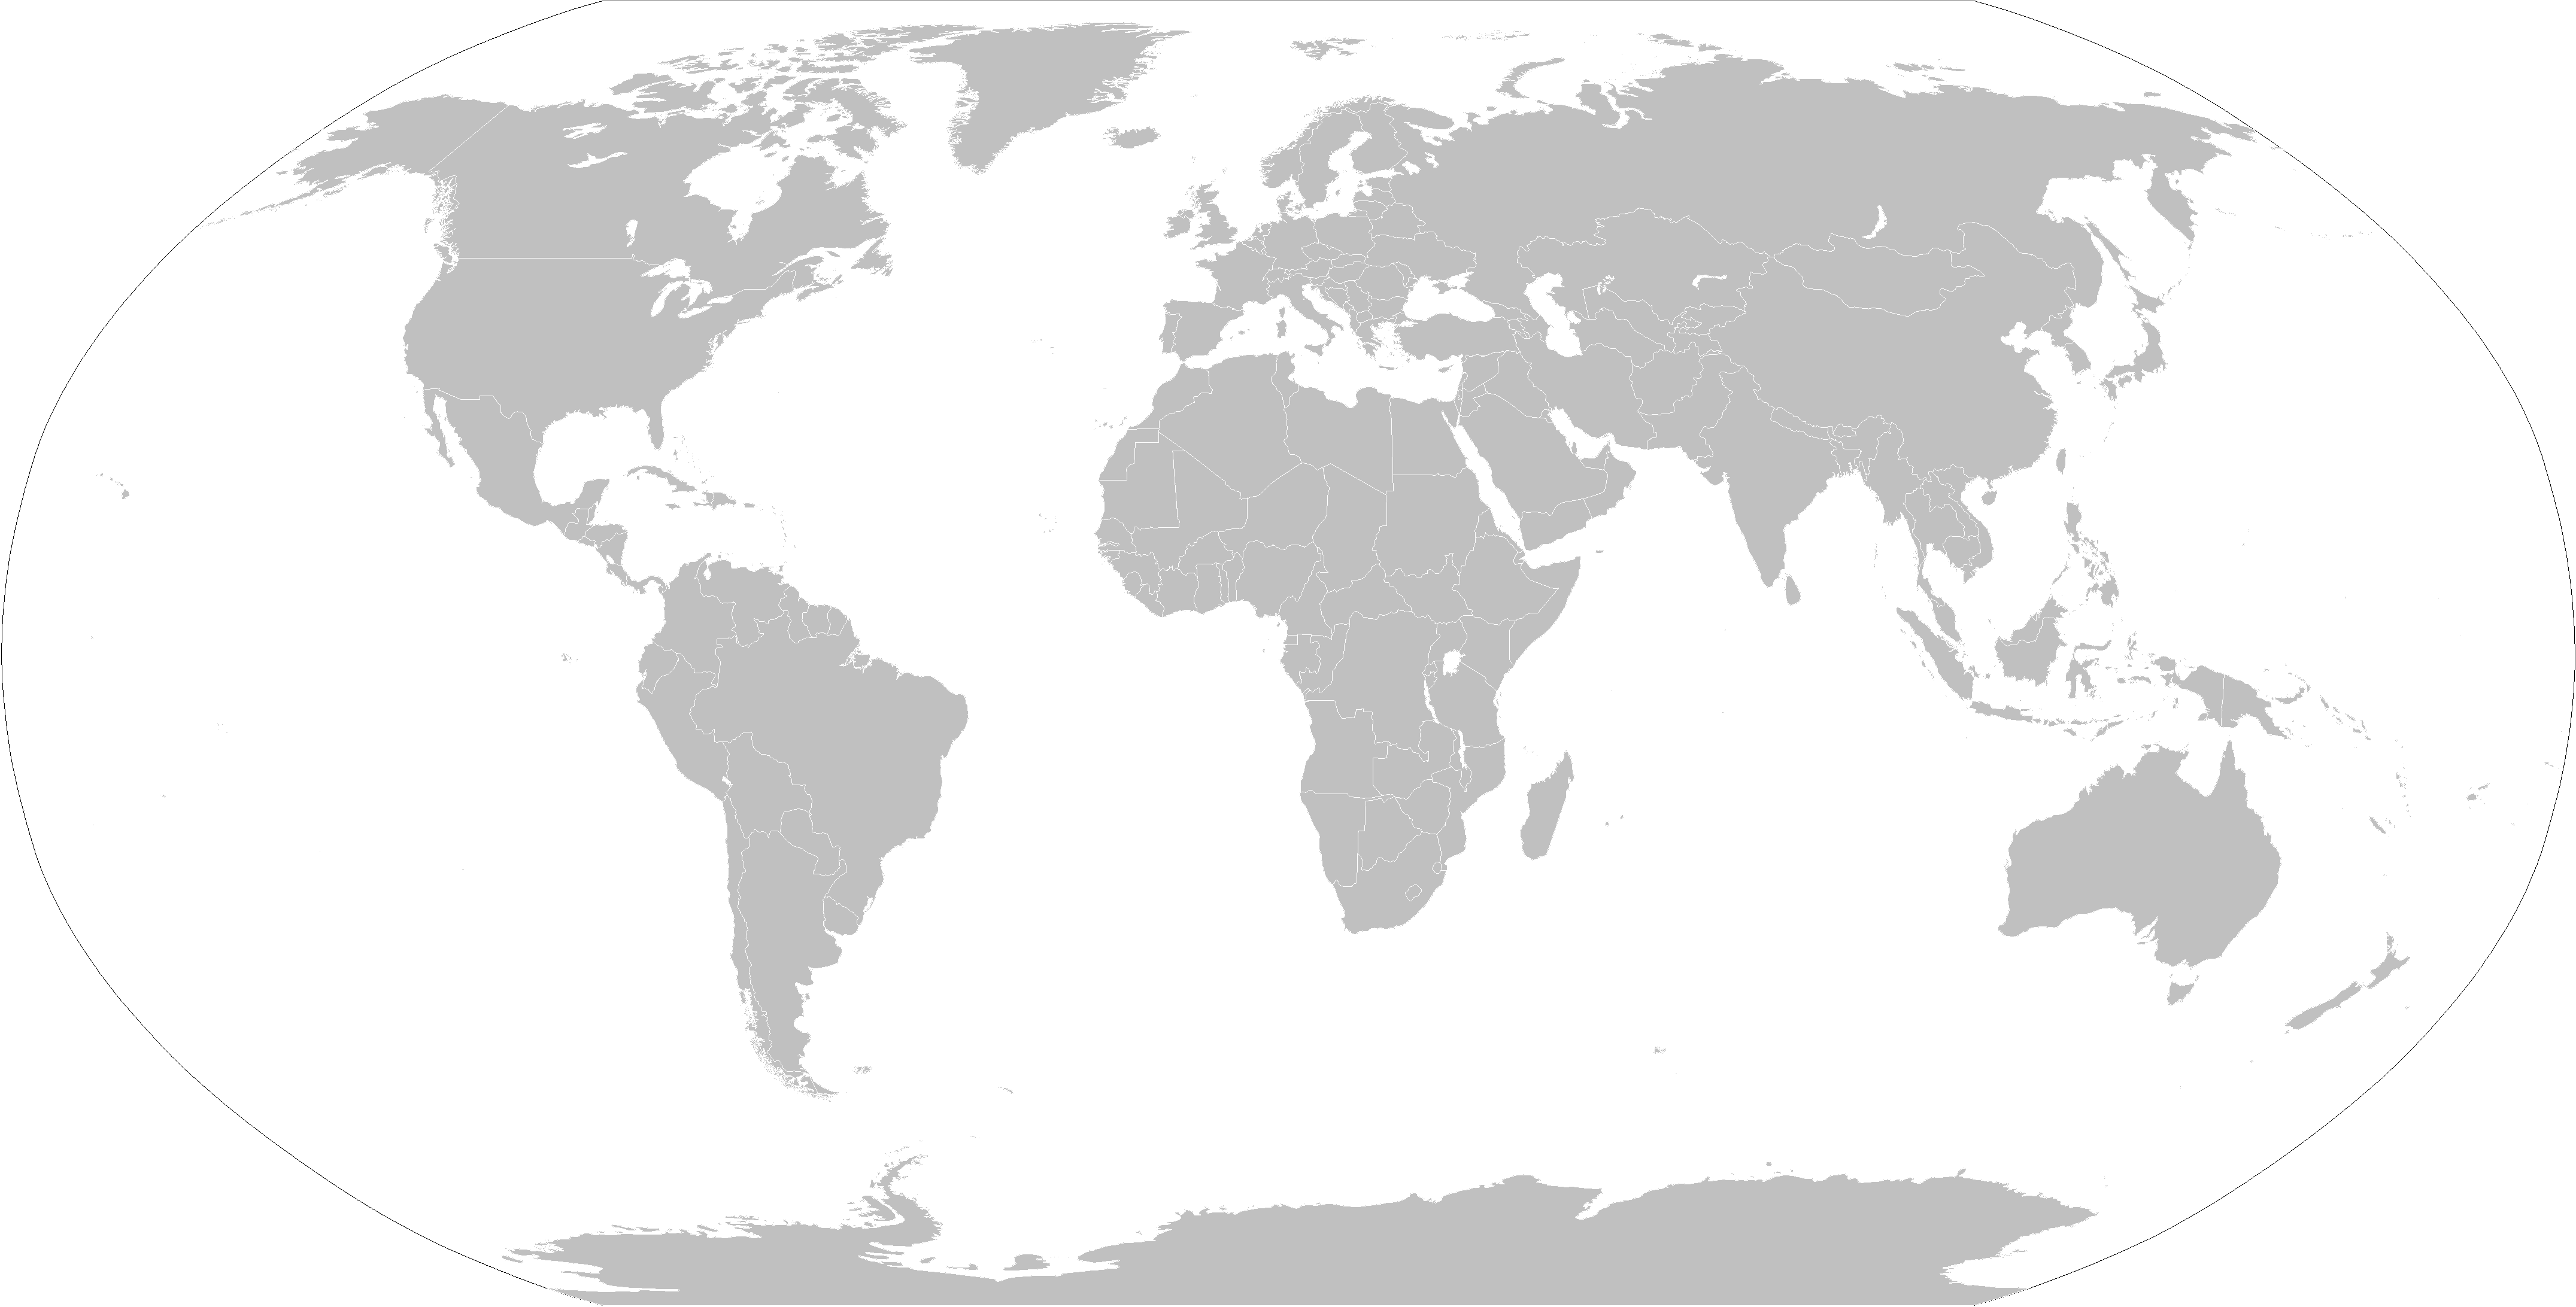
\includegraphics[width=\textwidth,
                             height=\textheight,
                             keepaspectratio]{
                pictures/world}};

        \node[color=accent] at (3.75, 6.25) {\faMapMarker*};
        \node[color=accent] at (3.75, 6.55) {
\includegraphics[width=0.045\textwidth,
                                                             height=0.045\textheight,
                                                             keepaspectratio]
                                                {pictures/distributors/digikey}};

        \node[color=accent] at (3, 5.8) {\faMapMarker*};
        \node[color=accent] at (3, 6.1) {
\includegraphics[width=0.04\textwidth,
                                                         height=0.04\textheight,
                                                         keepaspectratio]
                                                {pictures/distributors/arrow}};

        \node[color=accent] at (4.5, 6.25) {\faMapMarker*};
        \node[color=accent] at (4.5, 6.65)  {
\includegraphics[width=0.03\textwidth,
                                                            height=0.03\textheight,
                                                            keepaspectratio]
                                                {pictures/distributors/future-electronics}};

        \node[color=accent] at (11.825, 5.15) {\faMapMarker*};
        \node[color=accent] at (11.825, 5.55)  {
\includegraphics[width=0.03\textwidth,
                                                              height=0.03\textheight,
                                                              keepaspectratio]
                                                {pictures/distributors/lcsc}};

        \node[color=accent] at (3.4, 5.6)  {\faMapMarker*};
        \node[color=accent] at (3.4, 5.95) {
\includegraphics[width=0.03\textwidth,
                                                              height=0.03\textheight,
                                                              keepaspectratio]
                                                {pictures/distributors/mouser}};

        \node[color=accent] at (7.25, 6.6)  {\faMapMarker*};
        \node[color=accent] at (7.25, 6.95) {
\includegraphics[width=0.03\textwidth,
                                                              height=0.03\textheight,
                                                              keepaspectratio]
                                                {pictures/distributors/newark}};

        \node[color=accent] at (7.15, 6.5)  {\faMapMarker*};
        \node[color=accent] at (6.8, 6.55) {
\includegraphics[width=0.03\textwidth,
                                                              height=0.03\textheight,
                                                              keepaspectratio]
                                                {pictures/distributors/rs}};

        \node[color=accent] at (8, 6.5)  {\faMapMarker*};
        \node[color=accent] at (8, 6.9) {
\includegraphics[width=0.04\textwidth,
                                                          height=0.04\textheight,
                                                          keepaspectratio]
                                                {pictures/distributors/tme}};


        \node[color=accent] at (11.6, 4.2) {\faMapMarker*};
        \node[color=accent] at (11.6, 4.5) {
\includegraphics[width=0.066\textwidth,
                                                             height=0.05\textheight,
                                                             keepaspectratio]
                                                {pictures/distributors/element14}};

        \node[color=accent] at (12.125, 5.375) {\faMapMarker*};
        \node[color=accent] at (12.8, 5.375) {
\includegraphics[width=0.066\textwidth,
                                                               height=0.05\textheight,
                                                               keepaspectratio]
                                                {pictures/distributors/aliexpress}};

        \node[color=accent] at (12.7, 5.8) {\faMapMarker*};
        \node[color=accent] at (12.7, 6.15) {
\includegraphics[width=0.066\textwidth,
                                                               height=0.05\textheight,
                                                               keepaspectratio]
                                                {pictures/distributors/torex}};
    \end{tikzpicture}
\end{frame}

\subsection{BOM}
% Page de pièces de références (à copier-coller)
% Faire valider le BOM par quelqu'un d'autre
% Consolidation du BOM
% Un assemblage va coûter autant que les pièces
% Prix de vente = Fab price * 2.5 (eevblog)
% Limiter la taille du BOM (assemblage)
% Toujours tout mettre dans le BOM
%  - Fusibles
%  - Vis & Mechanical
%  - Alimentations
%  - Stencils!
% Quand utiliser des passives qui coûtent cher
